In this section, first, we explain how we evaluated MedChain's performance. Then, we present the evaluation results and discuss them. Finally, we describe MedChain limitations. 

\subsection{MedChain Simulations}
% A \textbf{very brief} introduction of simulation package of Cothority that is used in MedCahin. Provide some simulation results in this section and discuss them.

The simulation package of Cothority (Onet) can be used to run multiple code simulations on localhost, mininet, or deterlab and can be used to evaluate how implemented services and protocols work. We have defined and used simulations to evaluate MedChain's performance. 

We performed experiments on \textbf{localhost} in order to see if MedChain system scales well as the number of nodes in the network increases. To achieve this, we measured time the it takes to do various actions on a single query. More details about the evaluations is given in the following section. The code used to run simulations in MedChain can be found in \texttt{simulation/} directory of MedChain repository. In order to run simulations and reproduce the results presented here, you can use one of the following commands in \texttt{simulation/}:

\begin{verbatim}
    bash$ go test simul_test.go
\end{verbatim}

or 

\begin{verbatim}
    bash$ go build
    bash$ ./simulation service.toml 
\end{verbatim}

In fact, code in \texttt{simulation/service.go} and \texttt{simulation/service.toml} can be used to simulate a client talking to MedChain service.

\subsection{System Evaluation Setup and Results}

In order to evaluate the performance of MedChain system and understand if it scales well with increasing number of participating MedChain nodes in the network, we measured the time it takes to do various actions (see Table \ref{tbl:sim-actions}) on one query in network sizes of 5, 10, 20, and 30 MedChain nodes.

As it was mentioned earlier, simulations were run on localhost. Server CPU used is a 3.1 GHz Intel Core i7 with 16 GB of RAM. We have run 5 rounds of simulations with 5, 10, 20, and 30 nodes (hosts). 
% The communication bandwidth has been reduced to 100 Mb/s so that the results are more realistic. Also, a delay of 20ms is enforced between every 2 nodes (i.e., round-trip delay of 40 ms). 
Table \ref{tbl:sim-setup}, summarizes the setup used in simulations.
Figure \ref{fig:sim-plot-stacked} and Figure \ref{fig:sim-plot-logged} show the results of performance testing of MedChain service using simulations averaged over 5 rounds of simulations for a \textbf{single} query. The exact measurement values are recorded in Table \ref{tbl:sim-res}. Finally, in Table \ref{tbl:sim-actions}, we summarize what different actions in Table \ref{tbl:sim-res} and plots of results refer to.   

\begin{table}[ht]
\centering
\caption{MedChain Simulation Setup}
\label{tbl:sim-setup}
\begin{tabular}{ll}
Number of Simulation Rounds & 5\\
\hline
Number of MedChain Nodes & 5, 10, 20, or 30 \\
\hline
Branching Factor (BF) & 2 \\ 
\hline
%  Bandwidth & 100 Mbps\\
% \hline
 RunWait & 2h  \\
\hline
% Delay & 20 ms \\
% \hline
BatchSize & 5 \\
\hline
\end{tabular}
\end{table}

Please note that in Table \ref{tbl:sim-setup}, \textbf{Branching Factor} corresponds to the number of children each node has. \textbf{RunWait} corresponds to how long to wait for a run (one line of .toml-file in which we define simulations) to finish. 

% \textbf{Bandwidth} is the bandwidth in both sending and receiving direction for each MedChain node, measured in mega bits per second (Mbps). \textbf{Delay} is the delay between two hosts - the round-trip delay is thus twice this delay.  

\begin{table}[ht]
\centering
\caption{MedChain System Evaluation Results: Time measurements for various actions in MedChain averaged over 5 rounds for a single query}
\label{tbl:sim-res}
\begin{tabular}{|c|c|c|c|c|}
\hline
\textbf{Action} & \textbf{5 Nodes} & \textbf{10 Nodes} & \textbf{20 Nodes} & \textbf{30 Nodes}\\
\hline
prepare  & 48 $\mu$s & 38 $\mu$s & 34 $\mu$s & 254 $\mu$s \\ 
\hline
authorize  &5.13 s  & 7.20 s & 10.27 s & 14.36 s\\ 
\hline
reject & 3.02 s & 4.19 s & 7.21 s& 8.72 s\\ 
\hline
sign\_deferred & 0.85 s  &  1.52 s &  1.61 s & 2.63 s\\
\hline
execute\_deferred & 1.00 s & 1.24 s & 2.13 s & 2.45 s\\
\hline
round &  9.27 s & 12.69 s & 20.03 s& 26.57 s\\
\hline
\end{tabular}
\end{table}

\begin{table}[ht]
\centering
\caption{MedChain System Evaluation Results: Definition of actions measured. Step numbers referred to in this table correspond to steps of MedChain query workflow described in Section \ref{workflow-revisited} and illustrated in Figure \ref{fig:medchain_full_flow}}.
\label{tbl:sim-actions}
\begin{tabular}{|c|c|}
\hline
\textbf{Action} & \textbf{Definition}\\
\hline
\\[-1em]
prepare  &   \pbox{20cm}{Total time it takes to do steps 1 and 2\\[1pt]}\\ 
\hline
\\[-1em]
authorize   &   \pbox{20cm}{Total time it takes to do steps 3 , 4, 5, 6, and 7.\\[1pt]} \\ 
\hline
reject  &  Total time it takes to do steps 3, 4, and 5\\ 
\hline
sign\_deferred &  Total time it takes to do step 9   \\
\hline
execute\_deferred &  Total time it takes to do step 11 \\
\hline
round &  Total time it takes to do steps 1-12 (except for steps 8 and 10) \\
\hline
\end{tabular}
\end{table}

 \begin{figure}[htbp] 
        \centering 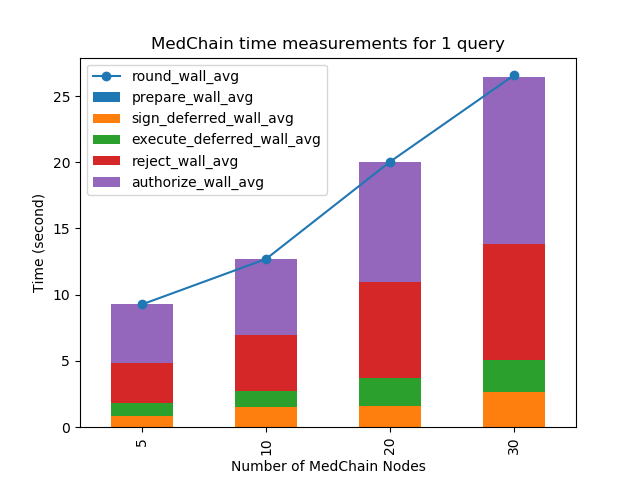
\includegraphics[width=1\columnwidth]{Images/barplot.png}
        \caption{\label{fig:sim-plot-stacked} 
         Medchain System Evaluation Results: Average wall time taken by various actions in MedChain (in seconds) vs. number of MedChain nodes in network. Actions are explained in Table \ref{tbl:sim-actions}. Measurement setup is described in Table \ref{tbl:sim-setup}. Please note that \textit{prepare\_wall\_avg} is so small that it is not depicted here. However, it is visible in plot of Figure \ref{fig:sim-plot-logged}, where time is shown in logarithmic scale. 
        }
\end{figure}

 \begin{figure}[htbp] 
        \centering 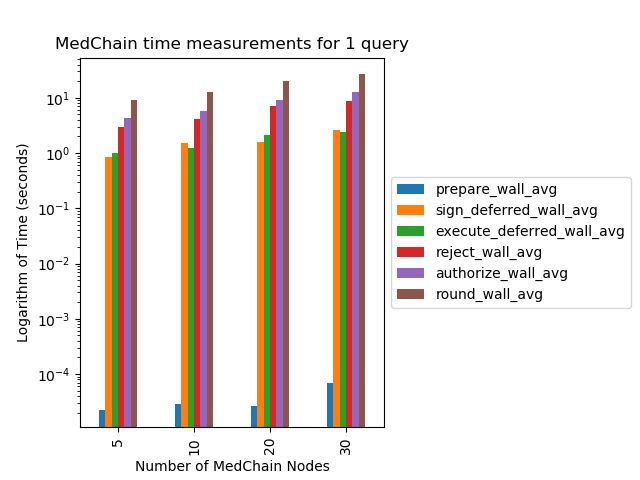
\includegraphics[width=1\columnwidth]{Images/barplot_log.png}
        \caption{\label{fig:sim-plot-logged} 
         Medchain System Evaluation Results: Logarithm of average wall time taken by various actions in MedChain (in seconds) vs. number of MedChain nodes in network. Actions are explained in Table \ref{tbl:sim-actions}. Measurement setup is described in Table \ref{tbl:sim-setup}.
        }
\end{figure}

\subsection{Discussions}

As it was mentioned earlier, we measured the time of various actions in MedChain for one query to understand if the service's performance scales well as the network size (number of MedChain nodes in the network) grows. Simulation results are illustrated in Figure \ref{fig:sim-plot-stacked} and Figure \ref{fig:sim-plot-logged}. Please note that in these plots, \texttt{xxx\_wall\_avg}, corresponds to the average time measured using the \textit{wall clock}. Wall clock measurements indicate the amount of time an external observer would have measured for a specific process to complete. So, if the system waits for a reply from the network, this waiting time is also included in the measurement. Please refer to \href{https://github.com/dedis/onet/tree/simul_docu/simul}{Onet Simulation library} for further details about its measurements. 

The results are averaged over 5 rounds of simulations using the setup described in Table \ref{tbl:sim-setup} for a single query.

Plots of Figures \ref{fig:sim-plot-stacked} and \ref{fig:sim-plot-logged} show exactly \textbf{the same measurement results}. However, since \textit{prepare\_wall\_avg} time was very small and was not shown in Figure \ref{fig:sim-plot-stacked}, logarithm of time measurements was used in Figure \ref{fig:sim-plot-logged}, so that \textit{prepare\_wall\_avg} is also illustrated. The actions measured and plotted in the figures are explained in Table \ref{tbl:sim-actions}. The exact time measurements are recorded in Table \ref{tbl:sim-res}.

According to the plots, we can see that, as expected, all processes take longer to complete as the network size (i.e., the number of MedChain nodes increases). Also, for every query, \textit{authorization} in MedChain is the longest process time-wise as it consists of more steps of the query workflow than the other processes (except for the full round); it also includes the time it takes for instance ID to be broadcast to the whole MedChain network which grows with the network size. The other observation is that, \textit{sign\_deferred} and \textit{execute\_deferred} take almost the same amount of time as they are both ByzCoin transactions on an instance of a deferred contract. However, \textit{execute\_deferred} action is likely to take more time than \textit{sign\_deferred} since it checks the signatures added to a proposed transaction as well as the Darc rules while the latter does not perform such checks on signatures while adding them. Furthermore, we observe that \textit{reject} action takes more time to complete than both \textit{sign\_deferred} and \textit{execute\_deferred} since it includes the time it takes for the ByzCoin to achieve consensus and add transactions to the ledger. As the sum of all actions equals the full round time, we conclude that MedChain service does not introduce time overheads in the workflow. 

Last but not least, we observe that the time of all actions increases almost linearly (in some cases sub-linearly) with number of nodes. Thus, we can conclude that the system exhibits scalability as number of MedChain nodes increases. However, it is important to note that, in reality, the time it takes for a query to be authorized by MedChain depends on the project Darc rules and the time it takes for all required users to sign a system deferred transaction so that the Darc rules are met. 

\subsection{Limitations}

\subsubsection{Darc Evolutions and Deferred Transaction Concurrency Issue}
We already discussed how Darcs are used to handle authorizations in MedChain. Also, in Section \ref{lbl:darcs}, we explained that rules in Darcs can be evolved and are, thus, Dynamic. Therefore, we can consider the case when a proposed deferred transaction of a query instance is awaiting the signature from user A before it can be executed by MedChain; in the meantime and before the query receives enough signatures it needs to be able to get executed, 2 system admins create (deferred) Darc evolution transactions to change the Darc rules governing the subject query instance synchronously. We can imagine that Darc evolution \#1 results in the rules for query to change in such as way that user A's signature is no longer needed and thus the query can be executed any time, while Darc evolution \#2 requests signatures from new users B and C so that the deferred query transaction can be executed. In this case, the order in which Darc evolution transactions are executed can change the final result state. For instance, if the Darc evolution \#1 is accepted first, the query can immediately be executed while this would not be the case with Darc evolution \#2 being accepted.

Another scenario in which such concurrency issues can happen is when a a deferred query transaction and a Darc evolution transaction of the Darc that governs the query are created concurrently. Again, depending on the order the two transactions are executed, the query can be rejected or authorized. 

This behavior is allowed in ByzCoin due to the fact that deferred transactions, such as the Darc evolution transaction, remain proposed until a threshold number of signatures are added to them and hence the time and order in which signatures are received for concurrent transactions matter. In order to prevent such synchronization issues, we need to implement concurrency control algorithms in either MedChain, or ByzCoin.   

% Discussion of some limitations of the server-side code as well the client-side code such as functionalities not supported \textit{in this version} of MedChain that are regarded as limitations (I do no have anything specific in mind yet)

% \textbf{Question}: Do you have any more ideas for this part?